Para ilustrar el uso de las herramientas desarrolladas utilizaremos como ejemplo
una aplicación bancaria, en la que los clientes de un banco pueden transferir
dinero de sus cuentas a otras cuentas propias o de terceros. 
Realizar una transferencia implica elegir dos cuentas, extraer el
monto indicado de la primera y depositarlo en la segunda. 
En cualquiera de los dos pasos de la transferencia (extraer y depositar) se
pueden producir errores.
Por ejemplo, el saldo puede ser insuficiente o el depósito puede superar el
máximo permitido.
La figura \ref{example} muestra las clases que implementan la lógica del
dominio.

	\begin{figure}[!h]
		\centering
		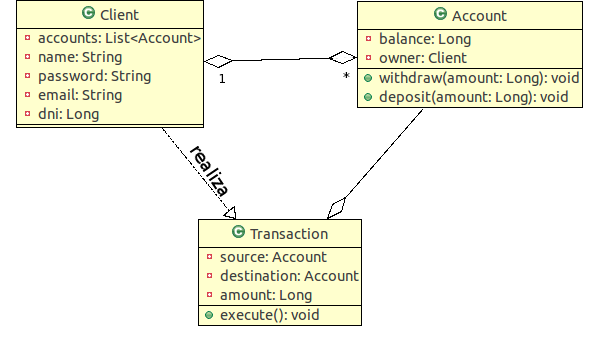
\includegraphics[scale=0.4]{img/transaccion}
		\caption{Diagrama UML de la aplicación de ejemplo}
		\label{example}
	\end{figure}	

A continuación se describirán las dos pantallas más importantes de la
aplicación, que nos permitirán mostrar las diferentes utilidades brindadas por
nuestra herramienta.
 
\begin{description}

	\item[Pantalla de Transferencia Simple]
		Esta primera pantalla permite elegir una de las cuentas propias, otra cuenta
		de cualquier cliente del sistema y realizar una transferencia de la
		primera hacia la segunda con el monto indicado. Esta pantalla se
		muestra en la figura \ref{trasferenciaSimple}.
		
		\begin{figure}[!h]
			\centering
			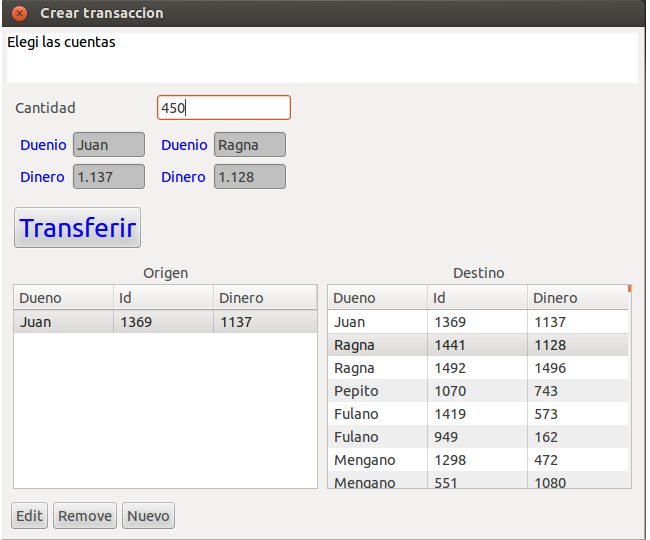
\includegraphics[scale=0.45]{img/simple-transferencia}
			\caption{Pantalla de transferencia simple}
			\label{trasferenciaSimple}
		\end{figure}

		Desarrollar esta utilidad con nuestra herramienta nos permite que el código
		solo se concentre en lo importante, que es debitar y extraer el monto. 
		La figura \ref{executeTransaction} muestra el método  \lstinline|execute| de la
		clase \lstinline|Transaction|. 
		Se puede ver que el código es limpio, no hay ningún comportamiento fuera de la lógica
		de negocio. 
		Además, no es necesario ningún manejo de excepciones. En caso de producirse un error, 
		la transacción en forma automática va a producir el \emph{rollback} de los cambios realizados.

		\begin{figure}[!h]
			\begin{lstlisting}
				public void execute(){
					this.source.withdraw(this.amount);
					this.destination.deposit(this.amount);
				}
			\end{lstlisting}
			\caption{Fragmento de código de la Clase Transaction}
			\label{executeTransaction}
		\end{figure}
		 
		
	\item[Pantalla de Transferencias Múltiples]
		Esta segunda pantalla nos permite realizar múltiples transferencias
		simultáneamente.
		A diferencia de la transferencia simple, se agrega una
		lista con las transferencias que se llevan a cabo.
		Aquí se puede apreciar la utilidad de las transacciones anidadas, dado que
		las transferencias pueden ser confirmadas o canceladas en su totalidad en
		cualquier momento. 
		La totalidad de las transacciones quedan firmes recién en el momento en el 
		que se acepta la operación principal. Esta pantalla se
		muestra en la figura \ref{trasferenciaMultiple}.
	
		\begin{figure}[hbt]
			\centering
			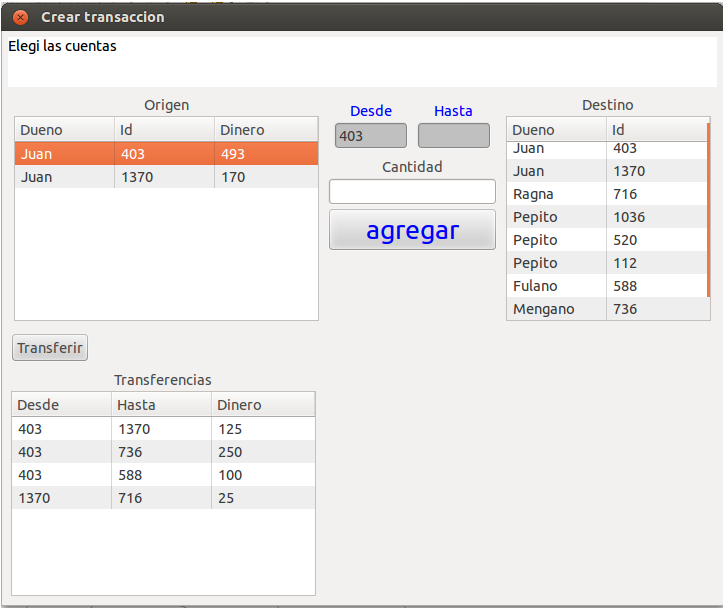
\includegraphics[scale=0.5]{img/multTransferencias}
			\caption{Pantalla de múltiples transferencias }
			\label{trasferenciaMultiple}
		\end{figure}
		
\end{description}